\documentclass{../SharedData/preziposters}
\usepackage[dutch]{babel}
\usepackage{../SharedData/brackets,../SharedData/Haskelllogo}
\usepackage[pdftitle={Poster Automaten en Berekenbaarheid},pdfauthor={Willem Van Onsem},pdfsubject={Berekenbaarheid},pdfkeywords={Turing, Reguliere Expressie, Automaten, Berekenbaarheid}]{hyperref}
\definecolor{redback}{rgb}{1,0.88,0.85}
\definecolor{greenback}{rgb}{0.9,0.98,0.85}
\definecolor{blueback}{rgb}{0.9,0.88,0.95}
\definecolor{orangeback}{rgb}{1.0,0.93,0.85}
\newcommand{\ssfunc}[1]{\ensuremath{#1:\left\{0,1\right\}^*\rightarrow\left\{0,1\right\}^*}}
\newcommand{\NNfunc}[1]{\ensuremath{#1:\NNN\rightarrow\NNN}}
\newcommand{\slang}[1]{\ensuremath{#1\subseteq\left\{0,1\right\}^*}}
\newcommand{\nlang}[1]{\ensuremath{#1\subseteq\left\{0,1\right\}^n}}
\newcommand{\sstri}[1]{\ensuremath{#1\in\left\{0,1\right\}^*}}
\newcommand{\nstri}[1]{\ensuremath{#1\in\left\{0,1\right\}^n}}
\newcommand{\cstri}[2]{\ensuremath{#1\in\left\{0,1\right\}^{#2}}}
\newcommand{\cc}[1]{\textbf{#1}}
\newcommand{\ccc}[1]{\textbf{#1}-\textit{complete}}
\newcommand{\cch}[1]{\textbf{#1}-\textit{hard}}
\newcommand{\cca}[2]{\ensuremath{\mbox{\cc{#1}}\left(#2\right)}}
\newcommand{\red}[1]{\ensuremath{\leq_{#1}}}
\newcommand{\xlogx}[1]{\ensuremath{#1\log\left(#1\right)}}

\newcommand{\constant}[1]{\ensuremath{\mathrm{#1}}}
\newcommand{\eulercon}[0]{\constant{e}}
\newcommand{\mnrel}[0]{\ensuremath{\sim_{\mbox{\small{mn}}}}}
\newcommand{\suprel}[0]{\ensuremath{\sim_{\mbox{\small{sup}}}}}
\newcommand{\langrel}[0]{\ensuremath{\sim_{L}}}

\DeclareDocumentCommand{\comput}{ O{LABEL} O{1.00} O{2.00} m m}{\def\cola{red};\def\colb{red};\ifthenelse{#5>1}{\def\cola{green};}{}\ifthenelse{\isodd{#5}}{\def\colb{green};}{}\computmul[#1][#2][#3]{#4}{\cola,\colb}}
\newcommand{\findcolor}[2]{\def#1{gray}\ifthenelse{\equal{#2}{TURING}}{\def#1{red}}{\ifthenelse{\equal{#2}{REGEX}}{\def#1{green}}{\ifthenelse{\equal{#2}{CTXFR}}{\def#1{blue}}{\ifthenelse{\equal{#2}{CTXSE}}{\def#1{purple}}{}}}}}
\DeclareDocumentCommand{\innerc}{ O{LABEL} O{1.00} O{2.00} m m m m m m }{\findcolor{\cola}{#4}\findcolor{\colb}{#5}\findcolor{\colc}{#6}\findcolor{\cold}{#7}\findcolor{\cole}{#8}\findcolor{\colf}{#9}\computmul[#1][#2][#3]{}{\cola,\colb,\colc,\cold,\cole,\colf}}

\newcounter{tmpA}
\newcounter{tmpB}

\title{Automaten en Berekenbaarheid}
\suptitle{Samenvatting van}
\author{W.~Van~Onsem\\KU~Leuven\\Departement~Computerwetenschappen\\Declaratieve~Talen~en~Artifici\"ele~Intelligentie~(DTAI)}
\disclaimer{\textbf{Disclaimer}: Er is geen garantie dat de volledige inhoud gedekt wordt of correct wordt voorgesteld.}

\begin{theposter}
\def\dma{5 mm};
\def\mid{594.5 mm};
\def\dyl{100.0 mm};
\def\dylm{5.0 mm};
\def\dylma{105.0 mm};
\def\dylhma{65.0 mm};
\def\dylqma{125.0 mm};
\def\dyw{1100.0 mm};
\def\dywb{550.0 mm};
\def\dywt{366.7 mm};
\def\dywq{275.0 mm};
\def\dywu{220.0 mm};
\def\dywh{183.3 mm};
\begin{scope}[yshift=-3*\dylm]
\begin{pgfonlayer}{background}

\defgroup[\dma][0][-\dylhma][
\includegraphics{pythia.pdf}]{\dyw}{0.6*\dyl}{Orakel (\S3.17)}{orange}{ORAKEL}
\defgroup[\dma][0][-\dylhma-\dylqma][
\includegraphics{turing.pdf}]{\dyw}{1.2*\dyl}{Turing (\S3.1-3.9)}{red}{TURING}
\defgroup[\dma][0][-\dylma-\dylhma-\dylqma][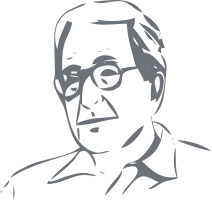
\includegraphics{chomsky.pdf}]{\dyw}{\dyl}{Context-sensitief (\S2.26)}{purple}{CTXSE}
\defgroup[\dma][0][-2*\dylma-\dylhma-\dylqma][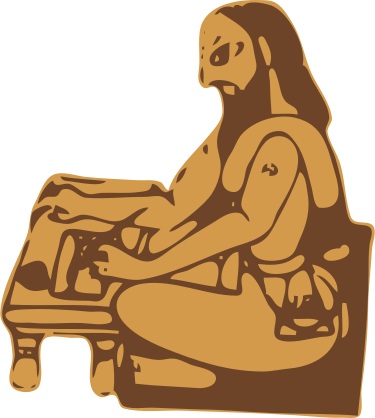
\includegraphics{panini.pdf}]{\dyw}{\dyl}{Context-vrij (\S2.19-\S2.25)}{blue}{CTXFR}
\defgroup[\dma][0][-2*\dylma-\dylhma-2*\dylqma][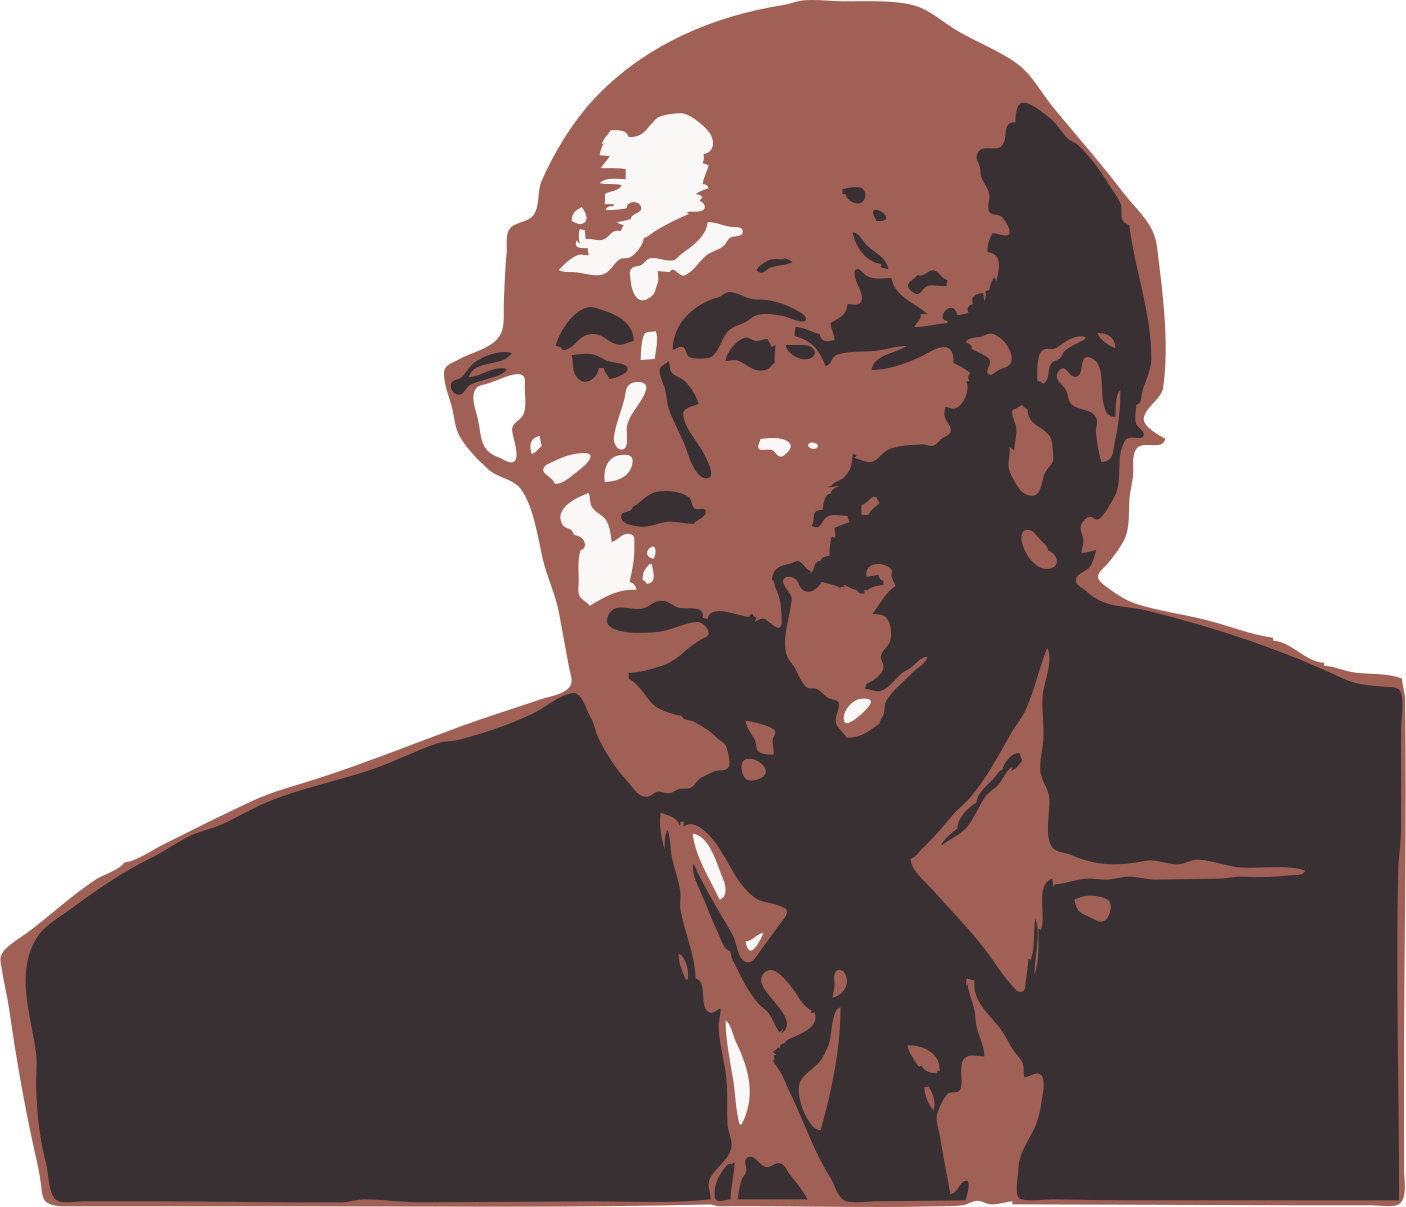
\includegraphics{rabin.pdf}]{\dyw}{1.2*\dyl}{Regulier (\S2.4-\S2.18)}{green}{REGEX}
\defgroup[\dma][0][-6*\dylma-5*\dma][\begin{tikzpicture}\haskelllogo\end{tikzpicture}]{0.8*\dyw}{\dyl}{Herschrijfsystemen ($\Lambda$-calculus; \S4)}{yellow}{LAMBDA}
\defgroup[\dma][0.8*\dyw+\dma][-6*\dylma-5*\dma][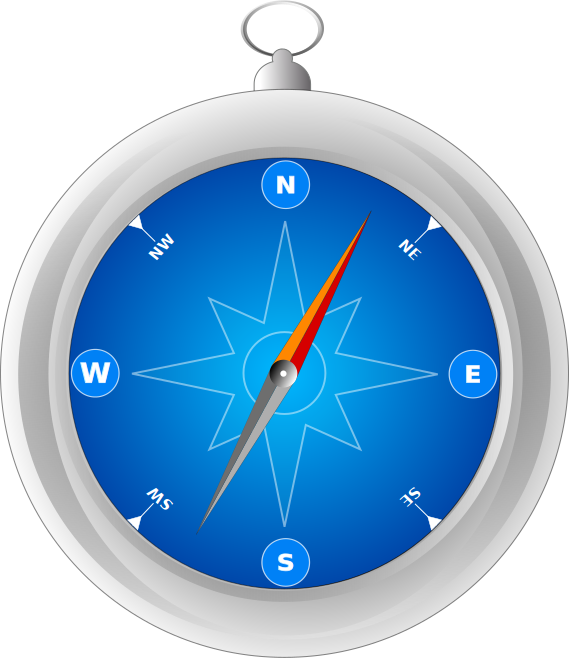
\includegraphics{compass.pdf}]{0.2*\dyw-\dma}{\dyl}{Legende}{backg}{LEGEND}
\defgroup[\dma][\dywh][-7*\dylma-5*\dma][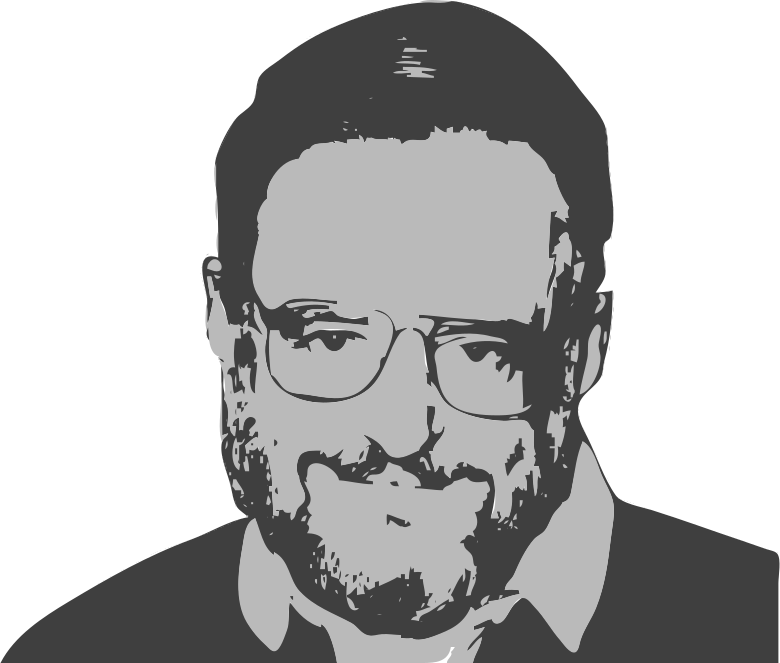
\includegraphics{conway.pdf}]{\dyw-\dywh-\dywt}{\dyl}{Andere paradigma's (\S5)}{gray}{OTHER}
\defgroup[\dma][0][-7*\dylma-5*\dma][
\includegraphics{kleene.pdf}]{\dywh}{\dyl}{Taal-aspecten (\S2.1-\S2.3)}{backg}{LANG}
\defgroup[\dma][\dyw-\dywt][-7*\dylma-5*\dma][
\includegraphics{godel.pdf}]{\dywt}{\dyl}{Problemen}{backg}{PROB}

\defgroupcols{REGEX}{A/0.0,B/22,C/63}{D/15.25,E/9.75,F/0.0};
\expandgroupcols{REGEX,CTXFR,CTXSE,TURING,ORAKEL}{A,B,C,D,E,F}

\grpvelef{TURING-T}{REGEX-B}{Chomsky hi\"erarchie (\S2-\S3)}
\grpholow{A}{B}{Beschrijven}
\grpholow{B}{C}{Automaten}
\grpholow{C}{D}{Representatiekracht}
\grpholow{D}{E}{Tijdscomplexiteit}
\grpholow{E}{F}{Berekenbaarheid}

\foreach \n in {B,C,D,E} {
  \draw[dashed,gray,thick] (COL-\n) -- (ORAKEL-LT -| COL-\n);
}

\foreach \c/\sb/\cmp/\toep in {REGEX/RE/n/{\item Extraheren van informatie\item Compilers\item Internetprotocollen\item Digitale elektronica},CTXFR/CFG/n^3/{\item Extraheren van informatie\item Compilers\item Natuurlijke taalverwerking},CTXSE/CSG/c^n/{\item Natuurlijke taalverwerking\item Webservers\item Gegevensbanken},TURING/TM//{\item Programmeertalen\item Levens redden (WO-II)},ORAKEL/O//{\item Filosofie\item Complexiteitstheorie}} {
  \coordinate (TMPR) at ($0.5*(\c-RB)+0.5*(\c-RT)$);
  \coordinate (TMPC) at ($0.5*(COL-D)+0.5*(COL-E)$);
  \ifthenelse{\equal{\cmp}{}}{\node (CC-\c-app) at (TMPR -| TMPC) {\parbox{5 cm}{Toepassingen:\begin{itemize}\toep\end{itemize}}};}{\node[scale=4.00] (CC-\c) at (TMPR -| TMPC) {\bigoh{\cmp}};\node[anchor=south] (CC-\c-t) at (CC-\c.north) {$s\in L_{\mbox{\small \sb}}$ wordt beslist in};\node[anchor=north] (CC-\c-app) at (CC-\c.south) {\parbox{5 cm}{Toepassingen:\begin{itemize}\toep\end{itemize}}};}
}
\end{pgfonlayer}
\CatchFileDef{\tempa}{defs.tex}{}
  \edef\tempb{\unexpanded{\foreach \l/\o/\x/\y/\twid/\xa/\xb/\xc in }{\unexpanded\expandafter{\tempa}}}
  \tempb {\titleminibox[(\o)][\l][\x][\y][\twid]{\xa}{\xb}{\xc}}

%Doorsnede/Unie/Complement/Concatenatie/Omkeren/Kleene-ster
\CatchFileDef{\tempa}{inner.tex}{}
  \edef\tempb{\unexpanded{\foreach \f/\fa/\fb/\fc/\fd/\fe/\ff in }{\unexpanded\expandafter{\tempa}}}
  \tempb {\begin{scope}[shift={(\f-C-LB)},xshift=1.5 cm,yshift=1.5 cm]\innerc{\fa}{\fb}{\fc}{\fd}{\fe}{\ff}\end{scope}}

\begin{scope}[shift={(LEGEND-LB)},xshift=4 cm,yshift=1.5 cm]\innerc[testlang]{TURING}{CTXSE}{CTXFR}{REGEX}{TURING}{CTXSE}\coordinate (L2L) at (-1.5,0);\coordinate (L2R) at (1.5,0);\end{scope}
\begin{scope}[shift={(LEGEND-LB)},xshift=8.5 cm,yshift=2.25 cm]\colorlegend[L2]{Turing-beslisbaar/red/a,Context-senstief/purple/b,Contextvrij/blue/c,Regulier/green/d}\end{scope}

\foreach \x/\t in {3/Complement,4/Concatenatie,5/Omkeren} {
  \draw[<-,thick] (testlang-S\x) -- (testlang-S\x -| L2R) node[anchor=west] (LX\x) {\t};
}
\foreach \x/\t in {1/Doorsnede,2/Unie,6/Kleene-ster} {
  \draw[<-,thick] (testlang-S\x) -- (testlang-S\x -| L2L) node[anchor=east] (LX\x) {\t};
}

\groupbox{(testlang-S1) (L2-a) (L2-b) (L2-c) (L2-d) (LX1) (LX2) (LX3) (LX4) (LX5) (LX6)}{Inwendige operator?}

\groupbox{(CCfiner) (CCmn)}{Myhill Nerode}

\end{scope}
\begin{scope}[shift={(PROB)},xshift=29 cm,yshift=-7.5 cm]
\comput[testlang][2.00]{$L$}{2}
\begin{scope}[xshift=-3 cm,yshift=-0.25 cm]\colorlegend[L1]{ja/green/a,nee/red/b}\end{scope}
\draw[<-,thick] (testlang-L) -- ++(-1.25,0) node[anchor=east] (LY1) {Taal};
\draw[<-,thick] (testlang-S1) -- ++(-1.25,0) node[anchor=east] (LY2) {Herkenbaar};
\draw[<-,thick] (testlang-S2) -- ++(1.25,0) node[anchor=west] (LY3) {Co-herkenbaar};
\end{scope}
\groupbox{(testlang) (L1-a) (L1-b) (LY1) (LY2) (LY3)}{Beslisbaar?}
\foreach \c/\sb/\co in {REGEX/RE/{A/2.00/3,H/2.00/3,E/2.00/3,Eq/2.00/3,Es/2.00/3,Regular/0.90/3,All/1.70/3}, CTXFR/CFG/{A/2.00/3,H/2.00/3,E/2.00/3,Eq/2.00/1,Es/2.00/3,Regular/0.90/0,All/1.70/1}, CTXSE/CSG/{A/2.00/3,H/2.00/3,E/2.00/1,Eq/2.00/1,Es/2.00/3,Regular/0.90/0,All/1.70/1},TURING/TM/{A/2.00/2,H/2.00/2,E/2.00/1,Eq/2.00/0,Es/2.00/2,Regular/0.90/0,All/1.70/0}} {
  \begin{scope}[shift={(\c-RT)},xshift=-7.5 cm,yshift=-2.5 cm]
  \setcounter{tmpA}{0}
  \setcounter{tmpB}{0}
  \foreach \l/\scl/\cmp in \co {
    \begin{scope}[xshift=2.5*\arabic{tmpA} cm,yshift=-2.5*\arabic{tmpB} cm]
    \comput[testlang][\scl]{\ensuremath{\mbox{\sc\l}_{\mbox{\tiny{\sb}}}}}{\cmp}
    \end{scope}
    \addtocounter{tmpA}{1}
    \ifthenelse{\value{tmpA}>2}{\setcounter{tmpA}{0}\addtocounter{tmpB}{1}}{}
  }
  \end{scope}
}
\end{theposter}
